\documentclass[11pt]{article}

\usepackage[margin=1.1in]{geometry}
\usepackage{amsmath}
\usepackage{booktabs}
\usepackage{graphicx}
\usepackage{microtype}
\usepackage[round]{natbib}
\usepackage[hidelinks]{hyperref}
\usepackage{caption}
\captionsetup{font=small, labelfont=bf, width=.94\textwidth}
\usepackage{orcidlink}
\usepackage{xcolor}

\newcommand{\code}[1]{\texttt{#1}}
\newcommand{\attested}{\textsc{attested}}

\title{AUSPEX: A Doctrine-Tagged, Source-Audited Corpus of\\
State-Sponsored Cyber Operations, with a Leakage-Aware\\
Who$\times$Why Engine and a Pre-Registered Forecast}

\author{Kara Zajac\,\orcidlink{0009-0001-7400-1394}\\
\small Black Flag Intelligence \quad \href{mailto:kara@soulstone.org}{kara@soulstone.org}}

\date{Draft of July 2026\thanks{Code, data, and every validation artifact:
\url{https://github.com/KaraZajac/AUSPEX}; frozen snapshot archived on Zenodo (DOI at release).
Live atlas and engine: \url{https://auspex.blackflagintel.com}. Released under CC~BY~4.0; layered
upstream attribution in \code{DATA-RIGHTS.md}.}}

\begin{document}
\maketitle

\begin{abstract}
\noindent Existing cyber-conflict datasets record \emph{who} attacked \emph{whom}, but not the
strategic \emph{why}: the doctrine under which an operation was tasked. We present \textbf{AUSPEX},
a corpus of \textbf{785} state-sponsored (and state-adjacent criminal) cyber events, each linked to
the strategic doctrines it advances, with per-claim primary sourcing, machine-verifiable schema, and
a published verification methodology. Every event has been audited claim-by-claim against its raw
cited sources under a documented six-point protocol; the audit reaches \textbf{100\% coverage}
(691 full, 94 partial). Doctrine links carry an evidentiary-confidence ladder and an
\emph{attacker/victim/defender} perspective tag, so who$\times$why analyses use only the attacker's own
doctrine. On this corpus we report three descriptive results and one engine. First, operations are
doctrinally \emph{legible} (76\% carry an attacker-rationale link) and \emph{follow} their doctrine in
time (median $+3$ years; 74\% of dated pairs postdate publication). Second, doctrine is
\emph{informative} about attribution: null-corrected mutual information is $1.67$ bits, cutting the
effective suspect pool $88\!\rightarrow\!28$ actors. Third, deterrence is \emph{not identifiable}
from an event atlas of this size --- we show why, rather than reporting a spurious effect. A
leakage-aware engine attains deployed attribution top-5 of 66.1\% (retrodictive) and 56.2\% on a
temporal holdout, and doctrine top-5 of 88.1\%, decisively above a naive baseline (3.4\%). Critically,
the completed audit \emph{lowered} every accuracy figure (attribution top-1 $64.9\!\rightarrow\!50.8$):
a de-circularization, not a regression. We pre-register six confirmatory predictions against
post-freeze data. The corpus, engine, harness, and this paper's figures are fully reproducible.
\end{abstract}

\section{Introduction}

Attribution answers \emph{who}. For a decade, cyber-conflict scholarship and threat intelligence have
converged on the who: named clusters (APT28, Lazarus, Sandworm), indictments, sanctions. But the
question a defender, a policymaker, or an examiner actually needs answered is \emph{why} --- under what
standing strategic frame was this operation tasked, and what does that frame predict next? Vendor
attribution names the who; strategic doctrine names the why; and only the join of the two is a usable
object. AUSPEX is built around that join.

Concretely, AUSPEX links each cyber event to the doctrines it advances: China's Military-Civil Fusion
and 2017 National Intelligence Law; Russia's information-confrontation and near-abroad postures; North
Korea's sanctions-evasion revenue plan; Iran's deniable-retaliation and forward-defense doctrines;
and so on across fifteen doctrine-authoring states. No prior public dataset carries these labels
(\S\ref{sec:related}). The contribution is four-fold:

\begin{enumerate}\itemsep2pt
\item \textbf{The dataset} (\S\ref{sec:data}): 785 events, 222 actors, 86 doctrines (199 pillars),
1{,}794 per-claim source records, on a formal JSON~Schema with an independent verification harness;
a Datasheet for Datasets \citep{gebru2021} accompanies the release.
\item \textbf{A verification census} (\S\ref{sec:census}): every event audited six-point against its
raw sources, 100\% coverage, with the status reported honestly (no ``verified'' overclaim) --- and,
unusually, we show the audit made the engine numbers \emph{worse} on purpose.
\item \textbf{Descriptive who$\times$why findings} (\S\ref{sec:results}): doctrinal legibility,
temporal precedence, doctrine$\rightarrow$actor information, and per-state modus-operandi fingerprints
--- each with the confounds it does and does not survive.
\item \textbf{A leakage-aware engine and a pre-registration} (\S\ref{sec:engine},
\S\ref{sec:prereg}): retrodictive and prospective attribution/doctrine prediction, and six
falsifiable predictions locked before the confirmatory data exists.
\end{enumerate}

We are deliberate about what the corpus is \emph{not}: it records \emph{disclosed} operations, not the
population of operations; its ground truth is analyst-concurred vendor attribution, not a verified
oracle; and its labels are analyst-mediated assessments. Every result below is framed by those limits,
which we treat as first-class (\S\ref{sec:limitations}).

\section{Related work}\label{sec:related}

The closest public datasets are the European Repository of Cyber Incidents
\citep[EuRepoC;][]{eurepoc}, the Dyadic Cyber Incident and Campaign Dataset
\citep[DCID;][]{valeriano2018}, the CFR Cyber Operations Tracker \citep{cfrtracker}, and the CSSM /
CISSM databases. These are strong on the \emph{who}, the \emph{when}, and coarse effect coding; DCID
in particular pioneered severity and objective coding for state dyads. What none of them carries is a
\emph{doctrine} label space --- a standing strategic frame, dated to a founding document, linked to
each operation with an evidentiary-confidence and perspective tag. AUSPEX's differentiators are
therefore: (i) doctrine links as a first-class label; (ii) per-claim sourcing with archived
content-hashes rather than a single citation per incident; (iii) a machine-verifiable schema plus a
published reliability and verification methodology; and (iv) a leakage-aware prediction engine
shipped alongside the data. On the modeling side, our attribution engine follows the class-imbalance
literature \citep{rennie2003}; the honest-evaluation posture (leave-one-out, temporal holdout,
null~$=$~miss, prose de-leaking) follows recent cautions on optimistic backtests in security ML.

\section{The dataset}\label{sec:data}

\paragraph{Scope and shape.} AUSPEX records 785 events across fifteen doctrine-authoring states
(US, RU, CN, IR, KP, IL, IN, PK, TR, BY, VN, UK, FR, KR, AE) plus a stateless \code{criminal} bucket
for financially-motivated crews. Of these, 648 are \emph{operations} (intrusion, theft, disruption,
influence, pre-positioning, cyber-physical) and 137 are \emph{meta} events (doctrine publications,
sanctions and attribution notices, law-enforcement actions) --- kept in the atlas and in engine
training, but excluded from the prediction label sets, since predicting the doctrine of a
doctrine-publication is circular. Figure~\ref{fig:corpus} shows the attributed operational corpus over
time: the familiar collection-driven post-2015 rise, and the shifting mix of China, Russia, Iran, DPRK,
and criminal activity.

\begin{figure}[t]\centering
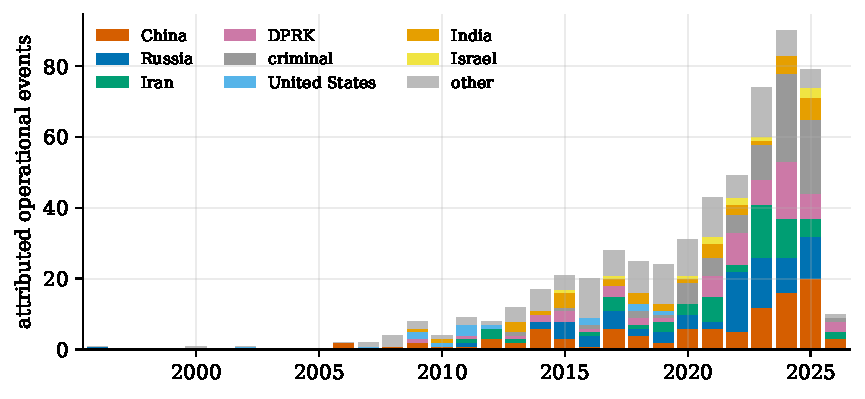
\includegraphics[width=.92\textwidth]{figures/fig-corpus.pdf}
\caption{Attributed operational events by attacker state and year (1996--2026). Counts are
collection-driven, not a census of the world; the corpus records disclosed, attributable operations.
``Other'' aggregates the eleven smaller doctrine-authoring states; unattributed operations are
omitted from this panel.}
\label{fig:corpus}
\end{figure}

\paragraph{Each event.} An event carries: a stable slug (never renamed; corrections add aliases);
\code{incident\_type}, \code{initial\_vector}, dates (operation start, disclosure, end, kept
distinct); attributions, each with an attributing organization, that organization's confidence, an
AUSPEX assessment, an attribution level (nation / named-actor / named-unit / activity-cluster), and a
source; targets; and \code{doctrine\_links}. Actor identifiers and aliases follow the MISP Galaxy
threat-actor clustering where it exists, reviewed on conflict \citep{mispgalaxy}. Every load-bearing claim links to a primary source
(government release, vendor report, court document, indictment); URLs are curl-verified, and where a
source is un-fetchable it is recorded \code{url:~null} with a note. We do not redistribute copyrighted
source bodies --- only the URL and a SHA-256 content hash (\code{content\_sha256}) are published, so a
third party can re-fetch and verify without AUSPEX re-hosting the text.

\paragraph{Doctrine links, confidence, and perspective.} A doctrine link records the
\code{doctrine\_id}, a pillar within it, a \code{confidence} on a three-rung ladder, a
\code{perspective}, and structured \code{inference\_basis} reasoning. The confidence ladder is
deliberately strict: a link is \attested{} \emph{only} when a cited source names the strategic goal in
substance (with a verbatim \code{source\_quote}); otherwise it is \code{strongly\_inferred} or
\code{plausible}, with the signals and ruled-out alternatives recorded. The perspective tag ---
\code{attacker-rationale}, \code{victim-response}, or \code{defender-response} --- is what makes the
who$\times$why analyses honest: Stuxnet is tagged with the US/Israeli \emph{attacker} doctrines and,
separately, with Iran's asymmetric-warfare doctrine as a \emph{victim-response}; only the former enter
any who$\times$why computation. Figure~\ref{fig:ladder} shows the resulting distribution. The
\attested{} stratum is small by construction --- 9\% of operations --- because it demands that a
\emph{source}, not the analyst, name the goal.

\begin{figure}[t]\centering
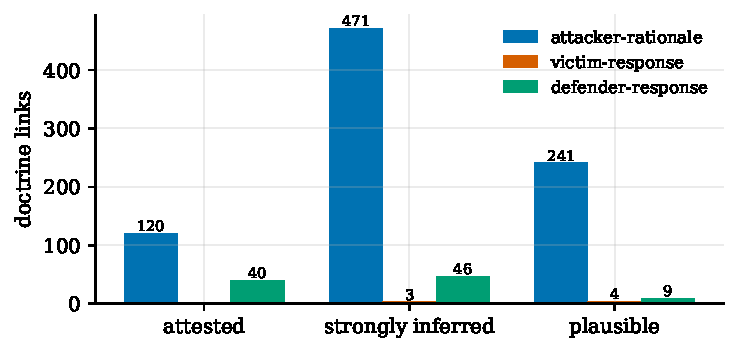
\includegraphics[width=.62\textwidth]{figures/fig-ladder.pdf}
\caption{Doctrine links by confidence and perspective. The strict \attested{} rung (a source names
the goal) is small on purpose; who$\times$why analyses restrict to \emph{attacker-rationale} links
and report the \attested{}-only cut as the honest robustness check.}
\label{fig:ladder}
\end{figure}

\section{The verification census}\label{sec:census}

The integrity backbone of the release is a human-directed, machine-executed audit of every event
against its raw sources. Under a documented six-point protocol --- (a)~facts, (b)~attribution,
(c)~dates, (d)~doctrine links, (e)~attribution level, (f)~actor identity, each checked against the
\emph{raw} source text, not the atlas prose --- each event was fetched, snapshotted (URL $+$ SHA-256),
corrected, and stamped. The audit is performed by a large language model (Claude Opus~4.8, recorded
per event as \code{verified\_by:~claude-opus-4.8}); this is a 100\%-coverage record-versus-source
audit, and we are careful to disclose it as such --- distinct from, and not implying, independent human
inter-rater verification, which is a separate reliability study. Coverage is \textbf{100\%}: 691
events \emph{full} (every load-bearing claim on a snapshotted source) and 94 \emph{partial} (a
load-bearing source was un-snapshottable --- bot-walled or link-rotted --- and was mirror-corroborated);
zero unstamped (Figure~\ref{fig:census}, right).

The census removed fabricated and duplicate events, merged duplicates, re-homed mis-dated events, and
stripped over-attestations and fabricated tradecraft throughout. Its most instructive effect is on the
engine (Figure~\ref{fig:census}, left): \emph{every} accuracy figure fell (attribution top-1
$64.9\!\rightarrow\!50.8$, doctrine $68.5\!\rightarrow\!62.8$, joint $47.9\!\rightarrow\!38.0$). This
is the audit working as designed. The removed events were disproportionately the over-clean,
over-attributed, or fabricated ones the engines had partly memorized; excising them
\emph{de-circularizes} the numbers. A dataset whose reported accuracy \emph{drops} after its authors
audit it is exhibiting the opposite of the optimism that inflates security-ML benchmarks.

\begin{figure}[t]\centering
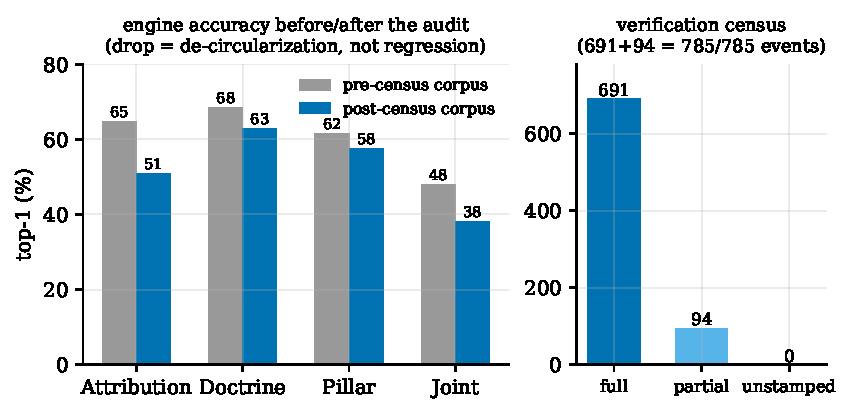
\includegraphics[width=.92\textwidth]{figures/fig-census.pdf}
\caption{The verification census. \emph{Left:} engine top-1 accuracy before and after the audit ---
every engine falls, a de-circularization (the audit removed over-attributed and fabricated events the
model had memorized), not a regression. \emph{Right:} 100\% coverage --- 691 full $+$ 94 partial of
785, zero unstamped.}
\label{fig:census}
\end{figure}

\section{Descriptive results: who$\times$why}\label{sec:results}

All results use attacker-rationale doctrine links, year granularity, and are computed by the
\code{analysis/} scripts (\code{make findings}); each figure regenerates from the atlas. We report both
the all-links and the strict \attested{}-only cut throughout, and name the confounds each survives.

\subsection{Operations are doctrinally legible and follow their doctrine}

\paragraph{Legibility.} 495 of 648 operations (76\%) carry at least one attacker-rationale doctrine
link. This is explicitly a \emph{tagging-coverage} measure, not a claim about the world's doctrinal
saturation: doctrines enter the atlas partly \emph{because} operations were observed
(selection on the dependent variable), so an operation that resists a doctrinal reading may simply not
get a link.

\paragraph{Precedence.} If doctrine merely rationalized operations after the fact, operations would
predate their documents. They do not. Across 468 (operation, dated-doctrine) pairs, the median gap is
$+3$ years and 74\% of pairs \emph{postdate} the document's publication (Figure~\ref{fig:precedence});
restricting to formally dated instruments (statute / strategy / treaty), $n=400$ pairs, median $+4$
years, 72\% follow. Precedence does not prove generation --- a state can codify what it already does ---
but it rules out the simplest reverse-causation story.

\begin{figure}[t]\centering
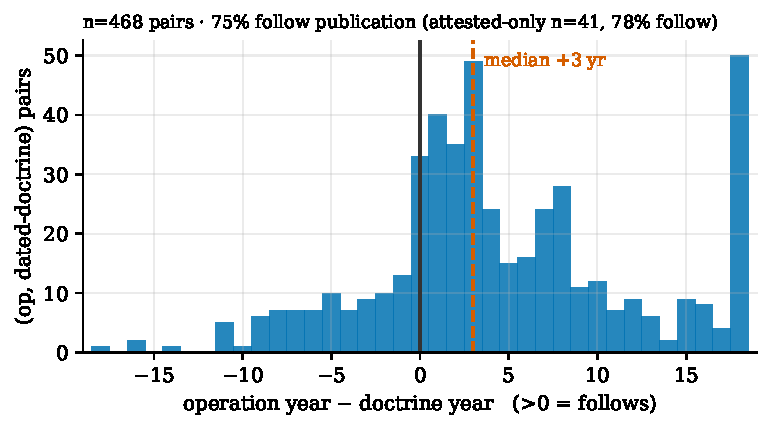
\includegraphics[width=.80\textwidth]{figures/fig-precedence.pdf}
\caption{Temporal precedence. Distribution of (operation year $-$ doctrine publication year) over
dated pairs. The mass sits to the right of zero: operations follow their doctrine (median $+3$~yr,
74\% follow). The small right-tail overflow is foundational doctrines (e.g. Israel's Begin Doctrine,
1981) paired with recent operations.}
\label{fig:precedence}
\end{figure}

\subsection{Doctrine is informative about attribution}

Knowing the doctrine narrows the actor. We measure this with mutual information, null-corrected by a
$K=40$ label permutation (the naive drop over-states narrowing $\sim\!6\times$ on a sparse corpus, so
we report only the corrected figure). Baseline actor entropy is $6.46$ bits; conditioning on doctrine
leaves $H(\text{actor}\mid\text{doctrine})$ such that null-corrected $\mathrm{MI}=1.67$ bits --- $26$\%
of actor uncertainty --- cutting the effective suspect pool from $88$ to $28$ actors
(Figure~\ref{fig:information}). The strict \attested{}-only cut gives $0.94$ bits ($20$\%,
$26\!\rightarrow\!14$): the same order of magnitude when a \emph{source}, not the analyst, names the
goal, so the relationship is not merely an artifact of how we chose to tag.

\begin{figure}[t]\centering
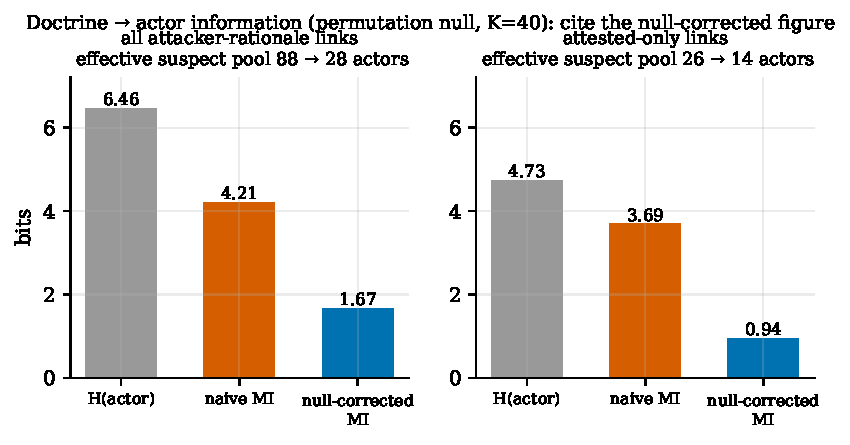
\includegraphics[width=.90\textwidth]{figures/fig-information.pdf}
\caption{Doctrine$\rightarrow$actor information. The naive mutual information (orange) is
sparsity-inflated; the null-corrected figure (blue, $K=40$ permutation) is the one to cite. Under both
the all-links and the strict \attested{}-only definition, knowing the doctrine resolves a fifth to a
quarter of actor uncertainty and roughly triples the resolving power of a suspect list.}
\label{fig:information}
\end{figure}

\subsection{States have distinct modus operandi}

Conditioning on the terminal outcome of an operation (data theft / systems denial / money / influence /
access) also carries state identity. Figure~\ref{fig:mo} shows each state's outcome fingerprint. China
is overwhelmingly data-theft (86\%); the profit-motivated buckets are unmistakable --- \code{criminal}
65\% money, DPRK 50\% money (the only \emph{state} above 25\% on money, a signature of the
sanctions-evasion revenue doctrine); Russia and Iran mix data-theft with a substantial denial /
disruption share (31\%, 35\%). Formally, $H(\text{state})$ falls from $3.54$ to $3.00$ bits given the
outcome (null $3.44$): modus operandi alone resolves 12\% of state identity beyond chance. As an actor
discriminator, outcome is real \emph{at the tails} (DPRK money is the sharpest signal in the corpus) but
weak on average, because espionage/data-theft is the universal default; a chained
doctrine$\rightarrow$target$\rightarrow$outcome narrowing is dominated by the doctrine term
($1.22$ null-corrected bits) and is under-powered at 493 single-actor events.

\begin{figure}[t]\centering
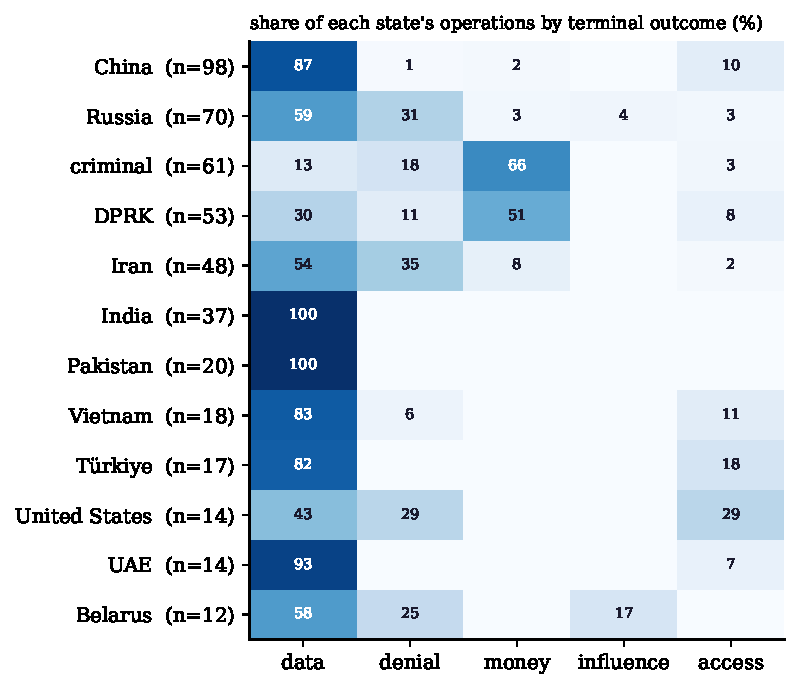
\includegraphics[width=.60\textwidth]{figures/fig-mo.pdf}
\caption{Per-state modus-operandi fingerprints: share of each state's single-actor, non-false-flag
operations by terminal outcome. The profit signature of \code{criminal} and DPRK, and the
data-theft dominance of China, India, Pakistan, and the UAE, are the sharpest structure.}
\label{fig:mo}
\end{figure}

\subsection{Deterrence is not identifiable --- and we say so}

A natural question is whether naming-and-shaming (indictments, sanctions, attributions) deters: does an
actor's operational tempo fall after a punitive action? We ran the event study honestly --- last
\emph{complete} year as the right-censoring boundary, tempo counted once per attacker-state --- and the
answer is that \emph{the design cannot answer it}. The 51 usable punitive actions collapse to
$n=4$ independent (state, window) clusters; the clustered difference-in-differences is $-0.69$ but the
sign test is non-significant ($p=0.62$), the estimator is endogeneity-biased \emph{toward} that sign
(actions respond to surges, which then mean-revert), and the control is contaminated by other treated
units (Figure~\ref{fig:deterrence}). We therefore publish the descriptive number with an explicit
refusal to read it as deterrence or defiance. The contribution here is methodological: an event atlas
of this size and structure cannot identify state-level naming-and-shaming effects, and pretending
otherwise is the error to avoid.

\begin{figure}[t]\centering
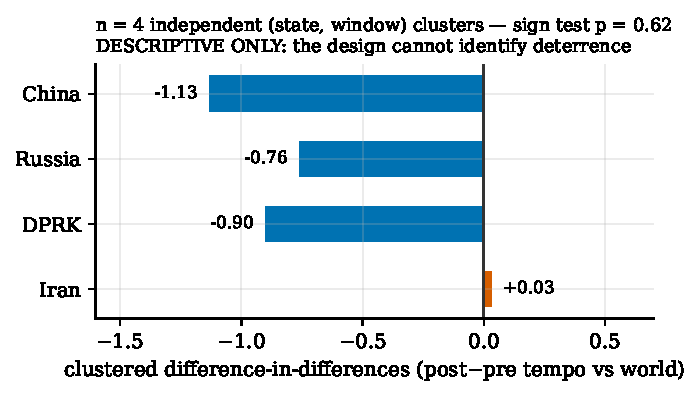
\includegraphics[width=.62\textwidth]{figures/fig-deterrence.pdf}
\caption{State-level deterrence, clustered to the effective sample. Four independent (state, window)
observations; a non-significant sign test ($p=0.62$); endogeneity biases toward apparent deceleration.
Published as \emph{descriptive only} --- the design is unidentified.}
\label{fig:deterrence}
\end{figure}

\section{The engine}\label{sec:engine}

Four prediction engines run over the atlas: attribution (actor), doctrine, pillar, and joint
(actor$\times$doctrine). Attribution is served by a ComplementNB base \citep{rennie2003} --- chosen for
the severe class imbalance of the one-and-few-event actor tail --- re-ranked by an L2 logistic stacker
over discriminative meta-features (named-operator and target-org overlap, malware-lineage hits, campaign
match, active-window). Doctrine and pillar use a multi-hot Naive Bayes. Features span target
sectors/countries, initial vectors, incident types, MITRE ATT\&CK techniques \citep{mitreattack} and co-occurrence pairs,
malware families with lineage partial-credit, named targets, geopolitical-marker proximity,
dyad-reactivity lag, editorial and algorithmic campaign clusters, and TF-IDF prose --- with a temporal
service prior (Empirical Bayes, $\lambda=0.2$) and temperature-scaled calibration.

\paragraph{Leakage discipline.} Every evaluation is leakage-aware. Prose features are scrubbed of actor
names/aliases \emph{and} doctrine-identifying tokens (the analyst who wrote a summary knew the answer);
a held-out event's own algorithmic campaign membership is suppressed while it is scored; and document
frequencies exclude the held-out event. We use the \textbf{null~$=$~miss} convention throughout: an
event whose only true label is a corpus singleton, unrankable under leave-one-out, counts as a miss,
not an exclusion, so numbers are comparable across engines and against the baseline.

\paragraph{Results.} Figure~\ref{fig:engine} reports top-5 hit rates under three regimes. Retrodictive
(leave-one-out / 5-fold CV) attribution reaches 66.1\% top-5 (deployed ComplementNB $+$ stack; top-1
50.8\%); doctrine 88.1\%, pillar 83.4\%, joint 56.9\%. The naive external baseline --- ranking actors by
a MITRE ATT\&CK Groups technique lookup --- scores 3.4\% top-5, so the engines are learning structure,
not exploiting a trivial prior. The honest prospective figure is the \textbf{temporal holdout} (train
$\le$ 2023-12-31, score 2024+): on the \emph{rankable} subset --- events whose true actor existed before
the split, the fair cold-start comparator --- attribution holds 56.2\% top-5 and doctrine 74.8\%;\footnote{The 56.2\% is the pre-registered reference-engine (multi-hot Naive Bayes) comparator, held fixed as the P6 target; the deployed ComplementNB\,$+$\,stack engine scores 56.9\% top-5 on the same rankable subset, so the deployed headline of $\approx$56\% is if anything conservative.}
counting cold-start new-actor events as misses, the all-test figures are lower (attribution 40.8\%),
which is the genuine cost of a fast-moving corpus stated plainly. Doctrine generalizes best through
time: the strategic frame an operation serves is the most temporally stable thing the engines predict,
which is precisely what makes it a candidate for forecasting.

\begin{figure}[t]\centering
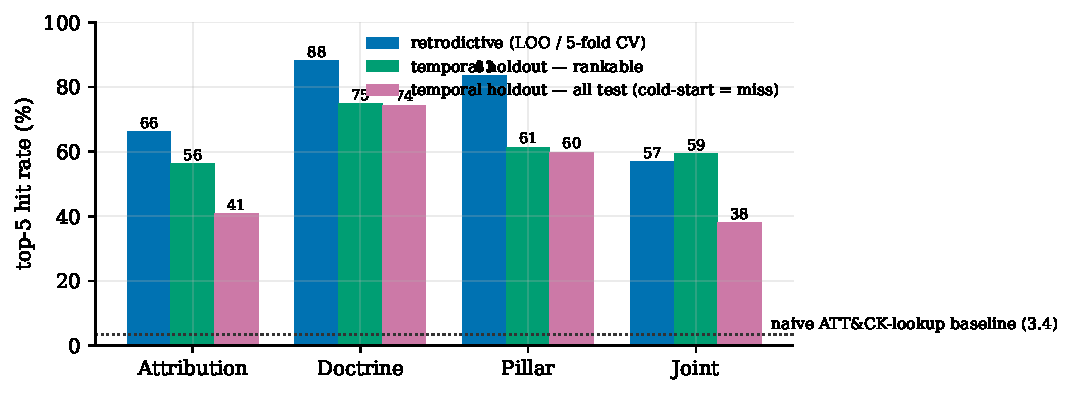
\includegraphics[width=.86\textwidth]{figures/fig-engine.pdf}
\caption{Engine top-5 accuracy under three regimes: retrodictive (LOO / 5-fold CV), temporal-holdout
rankable (true actor seen pre-2024), and temporal-holdout all-test (cold-start counted as miss). The
dotted line is the naive ATT\&CK-lookup baseline (3.4\%). Doctrine is the most temporally robust
target; attribution pays the largest retrodictive-to-prospective gap, as expected of a corpus that
adds new actors every year.}
\label{fig:engine}
\end{figure}

\section{Pre-registration}\label{sec:prereg}

Every result above is exploratory: discovered and tested on the same corpus. To convert the key claims
into falsifiable predictions, we pre-register six confirmatory predictions about events added to the
atlas \emph{after} the frozen snapshot, evaluated under unchanged tagging rules and analysis code
(Table~\ref{tab:prereg}). Thresholds are set deliberately below the current exploratory values to
allow sampling noise while remaining falsifiable; failed predictions will be \emph{reported},
interpreted (sampling noise vs.\ drift vs.\ claim wrong), not repaired. Two design notes reflect the
completed census: P5 is a single-state claim (China's National Intelligence Law dominance is clean;
Iran's operative doctrine is genuinely multipolar --- deniable-retaliation, forward-defense, and
resistance-axis run in parallel --- so Iran is reported exploratorily rather than pre-registered), and
P6 is scored on the rankable subset (true actor existed pre-freeze), whose current value ($56.2$\%)
clears the threshold but only narrowly, making it a genuine test rather than a lock.

\begin{table}[t]\centering\small
\begin{tabular}{@{}clcc@{}}
\toprule
\# & prediction on the post-freeze cohort & threshold & current \\
\midrule
P1 & doctrinal legibility ($\ge 1$ attacker-rationale link) & $\ge 65\%$ & 76\% \\
P2 & formal precedence (op postdates dated statute/strategy/treaty) & $\ge 60\%$ & 72\% \\
P3 & null-corrected $\mathrm{MI}(\text{actor};\text{doctrine})$ on pooled corpus & $\ge 1.0$ bits & 1.67 \\
P4 & DPRK financial-outcome share (only state $>25\%$) & $\ge 30\%$ & 50\% \\
P5 & China's post-pivot dominant doctrine stays \#1 (nat-intel-law-2017) & persists & clean \\
P6 & frozen engine, cold-start rankable attribution top-5 & $\ge 55\%$ & 56.2\% \\
\bottomrule
\end{tabular}
\caption{Pre-registered confirmatory predictions. ``Current'' is the exploratory value on the frozen
785-event corpus; thresholds sit below it. Locked at the freeze commit; the git history is the
timestamp.}
\label{tab:prereg}
\end{table}

\section{Limitations}\label{sec:limitations}

\textbf{Collection and disclosure bias.} The corpus records \emph{disclosed}, attributable operations,
skewed toward Western reporting; absolute tempo (Figure~\ref{fig:corpus}) reflects collection coverage,
which we measure with within-year normalization rather than assert away. \textbf{Ground-truth noise.}
Attribution labels are analyst-concurred vendor assessments, not a verified oracle; every accuracy
figure measures agreement with that consensus, which carries its own error rate. \textbf{Analyst-mediated
labels.} Doctrine links are AUSPEX assessments; the \attested{}-only cut is the honest one (a source
names the goal), and the machine census is a record-versus-source audit, not human inter-rater
verification --- an inter-rater $\kappa$ study is the standing next step. \textbf{Non-independence.}
Events cluster by campaign and actor, so i.i.d.\ bootstrap intervals are somewhat narrow (estimated
design effect $\approx 2$); a campaign-block bootstrap is future work. \textbf{Not causal.} Legibility,
precedence, and information are associations under the confounds named in \S\ref{sec:results}, not
evidence that doctrine \emph{generates} operations.

\section{Conclusion}

AUSPEX adds the missing axis to the study of cyber conflict: the strategic \emph{why}, as a
first-class, source-audited, machine-verifiable label joined to the operational \emph{who}. On a
corpus audited to 100\% coverage --- an audit that made our own numbers honestly worse --- operations
are doctrinally legible, follow their doctrine in time, and let doctrine cut the attribution suspect
pool roughly threefold; while deterrence, tested honestly, proves unidentifiable at this scale. The
corpus, the leakage-aware engine, the verification harness, and every figure in this paper regenerate
from public sources with a single command, and six predictions are locked against data that does not
yet exist.

\small
\bibliographystyle{plainnat}
\bibliography{refs}

\end{document}
